	%\documentclass[a4paper,12pt]{article}	
	%\documentclass[11pt]{book}
	\documentclass{report}
	\usepackage{amsmath} 
	\usepackage{amssymb}
	\usepackage{makeidx} 
	\usepackage{graphicx} 
	\usepackage[utf8]{inputenc}
	\usepackage[T1]{fontenc}
	\usepackage{textcomp}
	\usepackage{float}
	\usepackage[final]{pdfpages}
	

	%\usepackage{caption}
	%\usepackage{subcaption}
	%\usepackage{booktabs}


%\usepackage{mystyle} %Create your own file, mystyle.sty where you put all your own \newcommand statements, for example.

%\includeonly{chaptr2} %If you just want to process chaptr2.tex


	\begin{document}

	\author{Stefano Vergani}
	\title{Masters' Thesis}
	\date{June 2016}


\begin{titlepage}
    \begin{center}
        \vspace*{0.7cm}
        
        \Huge
        \textbf{Study of a Potential Third Time Component of Light in Liquid Argon}
        
    
        \vspace{1.5cm}


        \huge
	written by\\
        \textbf{Stefano Vergani}

	\vspace{3cm}
	\Large
       
        Submitted to the Department of Physics of ETH Z\"urich in partial fulfillment of the requirements for the degree of\\
        \textbf{Master of Science in Physics}
        
        \vspace{2cm}
        
        %\includegraphics[width=0.4\textwidth]{university}
        
        \Large
	Supervised by:\\
	\vspace{0.5cm}}
	Prof. Dr. Andr\'{e} Rubbia (ETHZ)\\
	Prof. Dr. Janet Conrad (MIT)\\
	Dr. Matthew Toups (FNAL)\\
	\vspace{0.75 cm}
        
        September 19, 2016
       
    \end{center}

\end{titlepage}
\afterpage{\null\newpage}

 \newpage

I declare that I have written this work by myself and have not used resources and materials besides those cited lege artis. Moreover, the present document has never been
submitted elsewhere. For this work, no degree, diploma or award has been conferred on me before, either at this or at any other institutions.
\bigskip

Hiermit erkl\"are ich, die eingereichte Arbeit selbständig verfasst und keine anderen als die von mir angegebenen Quellen und Hilfsmittel benutzt zu haben. W\"ortlich oder inhaltlich verwendete Quellen wurden entsprechend den anerkannten Regeln wissenschaftlichen Arbeitens zitiert. Ich versichere weiterhin, dass die vorliegende Arbeit nicht anderweitig eingereicht wurde.
\bigskip

\noindent Fermi National Accelerator Laboratory,\\   September 19, 2016
\cleardoublepage
\begin{abstract}

I describe here my Master's Thesis work, done in the Proton Assembly Building (PAB) at Fermi National Acceleration Laboratory, USA. My first task was to prepare and build an experiment for testing the new Hamamatsu Vacuum Ultra Violet (VUV) Multi Pixel Photon Counters (MPPC) in Liquid Argon (LAr). The test gave succeful results and an average amplified response of the MPPCs was obtained. The second part consisted in building an experiment for testing a hypotethical third intermediate component of scintillation light in Liquid Argon. The experiment, conducted in LAr,  measured the distributions of time differences between scintillation photons produced by an alpha source and measured by a VUV MPPC close to the source and two other MPPCs 65 cm away. One of those MPPC measured direct scintillation photons while the other measured waveshifted photons by a Tetra Phenyl Butadiene (TPB) coated plate. At the end of the data anaylsis we were not able to definitively confirm or refute the existence of a third time component fitting the data. Reasons and possible future steps are discussed. 

\end{abstract}


	\frontmatter
	\tableofcontents
%\include{./preface/preface}

	\mainmatter
		\chapter{First Approach with Pandora}

In this chapter it will explained how to run for the first time Pandora from a computer.

	\section{Run Pandora Blind} \label{sssec:pandora_blind}

In this part it is explained how to run for the first time Pandora using LArSoft and enabling the visualisation of the Pandora interface.  

\subsection{UBOONECODE}  \label{sssec:uboonecode}
As very first thing, the terminal must be opened. Digit then the following comand:

\begin{verbatim}
source /cvmfs/uboone.opensciencegrid.org/products/setup_uboone.sh
setup uboonecode v06_48_00 -q e14:prof
\end{verbatim}

The first command tells the computer to go to the CERN Virtual Machine File System (cvmfs) and to look for the setup file. This .sh file contains a certain amount of instruction for your computer and it has to be used everytime a new terminal is opened. The second command tells the computer which version of uboonecode has to be used. v06${\_}$48${\_}$00 is the current version as this notes are written but it is better always to check which is the latest version. Note that both command must be typed everytime a new terminal is opened. For further details about source files see Section \ref{sssec:setup}. Then type 

\begin{verbatim}

ls $UBOONECODE_DIR/job
cp $UBOONECODE_DIR/job/reco_uboone_mcc7_driver_stage2.fcl ./myreco_uboone_mcc7_driver_stage2.fcl

\end{verbatim}

The first command shows which files are contained in the directory ${\$}$UBOONECODE${\_}$DIR/job. It is worth knowing that the dollar symbol in front of UBOONECODE${\_}$DIR is an identifier, that means the name given to a certain path to a certain folder/file. Digiting

\begin{verbatim}

echo $UBOONECODE_DIR

\end{verbatim}

gives us the path to the folder, which in this case is

\begin{verbatim}

/cvmfs/uboone.opensciencegrid.org/products/uboonecode/v06_48_00

\end{verbatim}

The second command copies from the folder in the cvmfs the file .fcl on the local machine, changing the name of the copied file in myreco${\_}$uboone${\_}$mcc7${\_}$driver${\_}$stage2. 

%\begin{figure}[h]
%\scalebox{2}{\includegraphics[width=0.5\textwidth]{/home/stefano/Documents/fermilab/thesis/pictures/excitation}}
%\centering
%\caption{Schematic view of self-trapped exciton luminescence and recombination luminescence. They both produce scintillation light.}
%\label{fig:excitation}
%\end{figure}


	\subsection{FCL files}  \label{sssec:fcl_xml}

Fermilab Hierarchical Configuration Language (FHiCL or shortered FCL) is a language created at Fermi National Accelerator Laboratory (FNAL or Fermilab). For the pourpose of this guide, only few details will be given. For a proper introduction see \cite{fcl_guide}. Conceptually, the .fcl gives a list of instructions to the LArSoft software (\cite{larsoft}). Opening the .fcl file the file is this:

\begin{verbatim}

#include "reco_uboone_mcc7_driver_common.fcl"

process_name: McRecoAprStage2

services.DetectorClocksService.InheritClockConfig:  false

services.TFileService.fileName: "reco_stage_2_hist.root"
physics.reco: [ @sequence::microboone_reco_mcc7_stage2 ]
physics.trigger_paths: [ reco ]
outputs.out1.fileName: "%ifb_%tc_reco2.root"
outputs.out1.dataTier: "reconstructed"
source.inputCommands: ["keep *_*_*_*", "drop *_*_*_McRecoStage2" ]

\end{verbatim}

At this point, rename the process name at the second line as follow:

\begin{verbatim}

process_name: PandoraWorkshop

\end{verbatim}

After that, you can try to run LArSoft for the first time. Digit

\begin{verbatim}

lar -c myreco_uboone_mcc7_driver_stage2.fcl -n 5 /path/to/reco2/file.root 

\end{verbatim}

lar -c myreco${\_}$uboone${\_}$mcc7${\_}$driver${\_}$stage2.fcl launches the LArsoft using instructions given by the .fcl file. lar indicates that you want to run LArSoft, -c that you use the following .fcl file and -n 5 indicates to do certain processes looping on the first 5 events of the .root file and /path/to/reco2/file.root is the .root file you want to open and use. It does not indicate a specific file but rather any kind of .root file related to neutrino interaction in LAr you may have. A typical starting point is 

\begin{verbatim}

/pnfs/uboone/scratch/users/uboonepro/mcc7/v05_08_00/reco2/prodgenie_bnb_nu_uboone

\end{verbatim}

or, on Cambridge HEP systems

\begin{verbatim}

/r05/dune/mcproduction_v05_08_00/larsoft_output_reco2_bnb_nu/

\end{verbatim}

Any of the root files contained in those folders is good. Reco2 means the reconstruction has come to a further stage (hard reconstruction) whilst reco1 means a primary stage of reconstruction (low reconstruction). At the end of this process, a new .root file reco${\_}$stage${\_}$2${\_}$hist.root has been created with all the data related to the reconstructed events.  To visualize the reconstruced events with pandora software we need another piece, the .xml file. 

\subsection{XML files and Enable Visualisation}  \label{sssec:xml}  

Extensible Markup Language (XML) is a language used to give a set of rules in human and machine-readable format. Digit 

\begin{verbatim}

cp $UBOONECODE_DIR/scripts/PandoraSettings_MicroBooNE_Neutrino.xml ./MyPandoraSettings_MicroBooNE_Neutrino.xml

\end{verbatim}

to copy on your local machine the .xml file from the Uboonecode directory. The .xml will be the following:

\begin{lstlisting}[language=XML, caption=Python example]

<!-- Pandora settings xml file -->

<pandora>
    <!-- GLOBAL SETTINGS -->
    <IsMonitoringEnabled>false</IsMonitoringEnabled>
    <ShouldDisplayAlgorithmInfo>false</ShouldDisplayAlgorithmInfo>
    <SingleHitTypeClusteringMode>true</SingleHitTypeClusteringMode>

    <!-- PLUGIN SETTINGS -->
    <MuonPlugin>LArMuonId</MuonPlugin>

    <!-- ALGORITHM SETTINGS -->

    <!-- NEUTRINO-INDUCED EVENT RECONSTRUCTION -->
    <algorithm type = "LArListPreparation">
        <OnlyAvailableCaloHits>true</OnlyAvailableCaloHits>
        <OutputCaloHitListNameW>CaloHitListW</OutputCaloHitListNameW>
        <OutputCaloHitListNameU>CaloHitListU</OutputCaloHitListNameU>
        <OutputCaloHitListNameV>CaloHitListV</OutputCaloHitListNameV>
        <FilteredCaloHitListName>CaloHitList2D</FilteredCaloHitListName>
        <CurrentCaloHitListReplacement>CaloHitList2D</CurrentCaloHitListReplacement>
        <OutputMCParticleListNameU>MCParticleListU</OutputMCParticleListNameU>
        <OutputMCParticleListNameV>MCParticleListV</OutputMCParticleListNameV>
        <OutputMCParticleListNameW>MCParticleListW</OutputMCParticleListNameW>
        <OutputMCParticleListName3D>MCParticleList3D</OutputMCParticleListName3D>
        <CurrentMCParticleListReplacement>MCParticleList3D</CurrentMCParticleListReplacement>
        <MipEquivalentCut>0.</MipEquivalentCut>
    </algorithm>

    <algorithm type = "LArVisualMonitoring">
        <CaloHitListNames>CaloHitListW CaloHitListU CaloHitListV</CaloHitListNames>
    </algorithm>

...

\end{lstlisting}

and then modify the first lines as it follows:

\begin{lstlisting}[language=XML, caption=Python example]

<!-- Pandora settings xml file -->

<pandora>
    <!-- GLOBAL SETTINGS -->
    <IsMonitoringEnabled>true</IsMonitoringEnabled>
    <ShouldDisplayAlgorithmInfo>true</ShouldDisplayAlgorithmInfo>
    <SingleHitTypeClusteringMode>true</SingleHitTypeClusteringMode>

...

\end{lstlisting}

This will enable the visualisation. Now go back to the .fcl file and modify it adding the .xml file and enabling PandoraNu:

\begin{lstlisting}[language=C++, caption=Python example]

#include "reco_uboone_mcc7_driver_common.fcl"

process_name: PandoraWorkshop

#services.RottGraphicsEnablingService: {}

services.DetectorClocksService.InheritClockConfig:  false

services.TFileService.fileName: "reco_stage_2_hist.root"

physics.producers.pandoraWriter: @local::microboone_pandorawriter
physics.producers.pandoraWriter.HitFinderModuleLabel: "gaushit"
physics.producers.pandoraWriter.ConfigFile: "MyPandoraSettings_Write.xml"
physics.producers.pandoraNu.HitFinderModuleLabel: "gaushit"
physics.producers.pandoraNu.ConfigFile: "MyPandoraSettings_MicroBooNE_Neutrino.xml"

physics.reco: [ pandoraNu ]
physics.trigger_paths: [ reco ]
outputs.out1.fileName: "%ifb_%tc_reco2.root"
outputs.out1.dataTier: "reconstructed"
source.inputCommands: ["keep *_*_*_*", "drop *_*_*_McRecoStage2" ]

\end{lstlisting}

We use PandoraNu because it is the part of Pandora software used for reconstruction of neutrino events. Finally, with again the command

\begin{verbatim}

lar -c myreco_uboone_mcc7_driver_stage2.fcl -n 5 /path/to/reco2/file.root 

\end{verbatim}

the pandora interacting window will appear and man should be able to visualise the reconstructed events. 

\subsection{Pandora Interface}  \label{sssec:pandora_inter} 

At this stage, giving a comprehensive explanation of the interface is not worth it. Anyways, it is important to see that the user can controll manually which stage of the reconstruction she want to see. Launching the programm the first time gives the first stage of reconstruction (see Fig. \ref{fig:pandora}), whilst after pressing for the second time enter a further stage of reconstruction will be added (see Fig. \ref{fig:pandora2}).

\begin{figure}[h]
\scalebox{1}{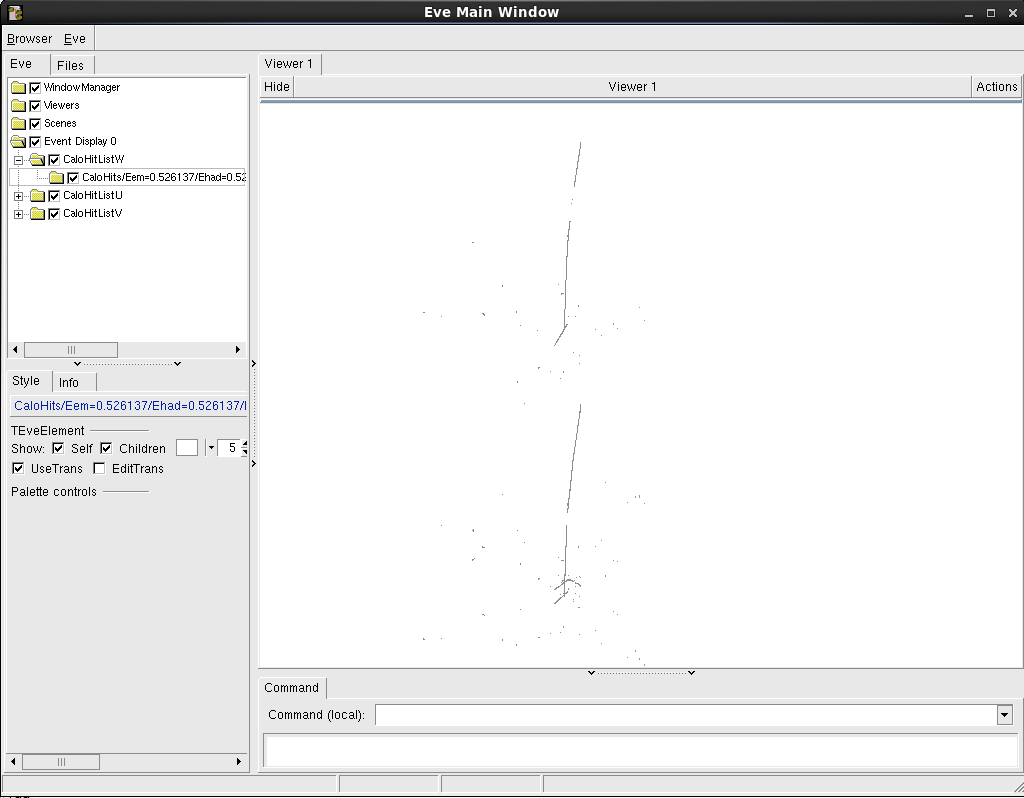
\includegraphics[width=0.5\textwidth]{/var/clus/usera/sv408/pandora_script/pandora}}
\centering
\caption{Pandora interface at first stage of reconstruction}
\label{fig:pandora}
\end{figure}

\begin{figure}[h]
\scalebox{1}{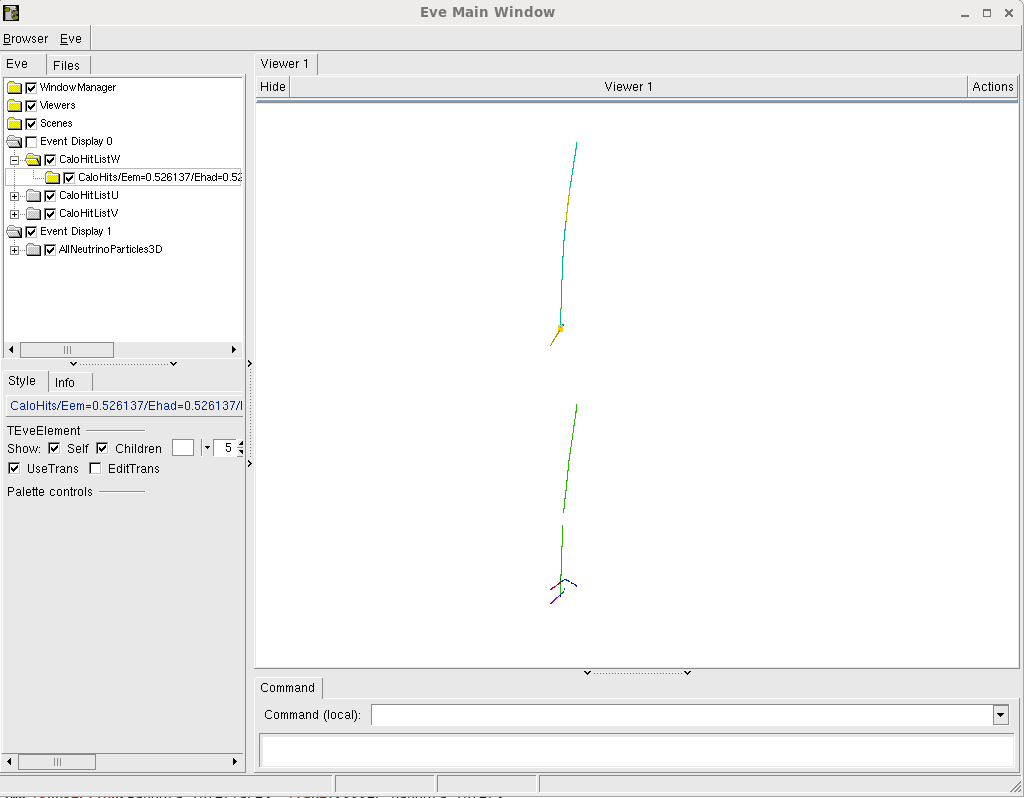
\includegraphics[width=0.5\textwidth]{/var/clus/usera/sv408/pandora_script/pandora_2}}
\centering
\caption{Pandora interface at second stage of reconstruction}
\label{fig:pandora2}
\end{figure}

\section{Write Events in Pandora Format} \label{sssec:intro}

Pandora uses special input objects (Hits, MCParticles, Gasps etc.). Those objects are already present in the .root file, but these files tends to come in a big size and for our pourposes we do not need all the information they contain. For this reason, it is possible to serialise input objects in .pndr files (which are small, but the portability is not guaranteed) or .xml files (which are large, but compressible). First thing to do is downloading a new .xml file which will give the command to write a .pndr file.

\begin{verbatim}

cp $LARPANDORA_DIR/scripts/PandoraSettings_Write.xml ./MyPandoraSettings_Write.xml

\end{verbatim} 

The file will be the following:

\begin{lstlisting}[language=XML, caption=Python example]

<!-- Pandora settings xml file -->

<pandora>
    <!-- GLOBAL SETTINGS -->
    <IsMonitoringEnabled>false</IsMonitoringEnabled>
    <ShouldDisplayAlgorithmInfo>false</ShouldDisplayAlgorithmInfo>
    <SingleHitTypeClusteringMode>true</SingleHitTypeClusteringMode>

    <!-- PLUGIN SETTINGS -->
    <MuonPlugin>LArMuonId</MuonPlugin>

    <!-- ALGORITHM SETTINGS -->
    <!--algorithm type = "LArEventReading">
        <EventFileName>INPUT_XML_OR_PNDR_FILE</EventFileName>
        <ShouldReadEvents>true</ShouldReadEvents>
        <SkipToEvent>0</SkipToEvent>
    </algorithm-->

     <algorithm type = "LArEventWriting">
        <EventFileName>Pandora_Events.pndr</EventFileName>
        <ShouldWriteEvents>true</ShouldWriteEvents>
        <ShouldOverwriteEventFile>true</ShouldOverwriteEventFile>
        <ShouldWriteMCRelationships>true</ShouldWriteMCRelationships>
        <ShouldWriteTrackRelationships>true</ShouldWriteTrackRelationships>
    </algorithm>
</pandora>

\end{lstlisting}

edit line 20 as it follows, if for example you want as an output the file "MyPandoraEvents.pndr":

\begin{verbatim}

<EventFileName>MyPandoraEvents.pndr</EventFileName>

\end{verbatim}

Then modify myreco${\_}$uboone${\_}$mcc7${\_}$driver${\_}$stage2.fcl as well:

\begin{verbatim}

physics.reco: [ pandoraNu, pandoraWriter]

\end{verbatim}

At this point, launch

\begin{verbatim}

lar -c myreco_uboone_mcc7_driver_stage2.fcl -n 5 /path/to/reco2/file.root 

\end{verbatim}

and in your folder the file MyPandoraEvents.pndr will be created.
%\afterpage{\null\newpage}

\afterpage{\null\newpage}
		\chapter{A New Algorithm}

In this chapter it will explained how to run for the first time Pandora from a computer locally. In the previous chapter, the exercises have been done using the LArSoft stored in the Fermilab servers. At the end of this section, the student will have her/his own version of Pandora stored locally. 

	
\section{Run Pandora Locally}

In this chapter it will explained how to run for the first time Pandora from a computer locally.


\subsection{Setup} \label{sssec:setup} 

As first thing, digit the following commands:

\begin{verbatim}

export MY_TEST_AREA=/path/to/your/test/area
export PANDORA_PFA_VERSION=v03-06-00
export ROOT_CMAKE_MODULE_PATH=/path/to/your/FindROOT.cmake/file

\end{verbatim}

This is to set the identifiers MY${\_}$TEST${\_}$AREA, ROOT${\_}$CMAKE${\_}$MODULE${\_}$PATH and PANDORA${\_}$PFA${\_}$VERSION (to see what is an identifier go to Section \ref{sssec:uboonecode}). With Pandora PFA we mean Pandora Particle Flow Algorithm,which is the GitHub name for Pandora \cite{pandora_doc}. It is worth noting that whilst the first area could be any possible folder you like, the Pandora version and the path to the Root cmake must be choosen wisely. For the version of a software it is always a good idea to try the latest version (for Pandora can be found here \cite{pandora_doc}). If it gives problems, simply try the recommended version or older ones. The path to the Root cmake interely dipends on where you saved Root. If you want to use Root stored in Fermilab

\begin{verbatim}

export ROOT_CMAKE_MODULE_PATH=$ROOTSYS/etc/cmake/FindROOT.cmake

\end{verbatim}

If you now try an echo command, it should give you back the path you indicated. One should type these three commands everytime a new terminal is opened. To avoid that, there are two possible options. The first one is to create a script, called for example setup.sh. This script will contain those three commands and typing 

\begin{verbatim}

source setup.sh

\end{verbatim}

the commands will be launched. There is also the possibility to launch automatically these commands. Go to your home directory and modify the file .bashrc. This file contain all the commands the terminal automatically run when it is opened. One can simply add the three exports, but this is not always the best thing to do because not always we want all these commands to be run automatically. So another option is to type:

\begin{verbatim}

alias start='source path/to/your/setup.sh'

\end{verbatim}

With this command, everytime one will digit "start" the command source setup.sh will be launched.

\subsection{Installation} \label{sssec:installation} 

Digit

\begin{verbatim}

cd $MY_TEST_AREA
git clone 
git clone https://github.com/PandoraPFA/PandoraPFA
cd PandoraPFA
git checkout $PANDORA_PFA_VERSION

\end{verbatim}

After this, you will have cloned the github repository on your machine. at this point create a folder to build Pandora

\begin{verbatim}

mkdir build
cd build

\end{verbatim}

and create the cmake file

\begin{verbatim}

cmake -DCMAKE_MODULE_PATH=$ROOT_CMAKE_MODULE_PATH \
-DPANDORA_MONITORING=ON -DPANDORA_LAR_CONTENT=ON  \
-DCMAKE_CXX_FLAGS=-std=c++14 ..

\end{verbatim}

the last command, -DCMAK${\_}$CXX${\_}$FLAGS=-std=c++14 orders to use the latest compiler avaible or at least version 14. The double dots at the end tells the compiler to search the file outside the directory "build".

Now it is possible to install Pandora locally

\begin{verbatim}

make -j4 install

\end{verbatim}

The installation process should take a couple of minutes. After that, we will setup a library and applicatio explicity tailored for the next exercises.

\begin{verbatim}

cd $MY_TEST_AREA
git clone https://github.com/PandoraPFA/WorkshopContent
cd WorkshopContent
mkdir build
cd build

cmake -DCMAKE_MODULE_PATH="$ROOT_CMAKE_MODULE_PATH;$MY_TEST_AREA/PandoraPFA/cmakemodules" \
-DPandoraSDK_DIR=$MY_TEST_AREA/PandoraPFA -DPANDORA_MONITORING=ON                         \
-DPandoraMonitoring_DIR=$MY_TEST_AREA/PandoraPFA                                          \
-DLArContent_DIR=$MY_TEST_AREA/PandoraPFA -DCMAKE_CXX_FLAGS=-std=c++14 ..

make -j4 install

\end{verbatim}

\section{Adding a new Algorithm} \label{sssec:new_algorithm}

In this part we will create a new algorithm. To do so we have to go in the subfolder Algorithms. There is already a set of templates which can be used. Digit

\begin{verbatim}

cd $MY_TEST_AREA/WorkshopContent/workshopcontent/Algorithms
python CreateNewAlgorithm.py --name MyTest

\end{verbatim}

The last command will create a new algorithm called MyTestAlgorithm (both .cc and .h files) using the existing templates. Now digit 

\begin{verbatim}

cd ..
cd Test

\end{verbatim}

and modify the file PandoraWorkshop.cc adding the parts in red:

\begin{lstlisting}[language=C++, caption=Python example]

...

#include "Api/PandoraApi.h"

#include "larpandoracontent/LArContent.h"
#include "larpandoracontent/LArPlugins/LArPseudoLayerPlugin.h"
#include "larpandoracontent/LArPlugins/LArRotationalTransformationPlugin.h"

\textcolor{red}{#include "workshopcontent/Algorithms/MyTestAlgorithm.h"}

#ifdef MONITORING
#include "TApplication.h"
#endif

...

int main(int argc, char *argv[])
{
    try
    {
        Parameters parameters;

        if (!ParseCommandLine(argc, argv, parameters))
            return 1;

#ifdef MONITORING
        TApplication *const pTApplication = new TApplication("Workshop", &argc, argv);
        pTApplication->SetReturnFromRun(kTRUE);
#endif
        const pandora::Pandora *const pPandora = new pandora::Pandora();

        PANDORA_THROW_RESULT_IF(pandora::STATUS_CODE_SUCCESS, !=, LArContent::RegisterAlgorithms(*pPandora));
        PANDORA_THROW_RESULT_IF(pandora::STATUS_CODE_SUCCESS, !=, LArContent::RegisterBasicPlugins(*pPandora));
        PANDORA_THROW_RESULT_IF(pandora::STATUS_CODE_SUCCESS, !=, PandoraApi::SetPseudoLayerPlugin(*pPandora, new lar_content::LArPseudoLayerPlugin));
        PANDORA_THROW_RESULT_IF(pandora::STATUS_CODE_SUCCESS, !=, PandoraApi::SetLArTransformationPlugin(*pPandora, new lar_content::LArRotationalTransformationPlugin));

\textcolor{red}{PANDORA_THROW_RESULT_IF(pandora::STATUS_CODE_SUCCESS, !=, PandoraApi::RegisterAlgorithmFactory(*pPandora, "MyTestAlgorithm", new workshop_content::MyTestAlgorithm::Factory));}

        PANDORA_THROW_RESULT_IF(pandora::STATUS_CODE_SUCCESS, !=, PandoraApi::ReadSettings(*pPandora, parameters.m_pandoraSettingsFile));

        int nEvents(0);
        while ((nEvents++ < parameters.m_nEventsToProcess) || (0 > parameters.m_nEventsToProcess))
        {
            if (parameters.m_shouldDisplayEventNumber)
                std::cout << std::endl << "   PROCESSING EVENT: " << (nEvents - 1) << std::endl << std::endl;

            PANDORA_THROW_RESULT_IF(pandora::STATUS_CODE_SUCCESS, !=, PandoraApi::ProcessEvent(*pPandora));
            PANDORA_THROW_RESULT_IF(pandora::STATUS_CODE_SUCCESS, !=, PandoraApi::Reset(*pPandora));
        }

        delete pPandora;
    }
    catch (pandora::StatusCodeException &statusCodeException)
    {
        std::cerr << "Pandora Exception caught: " << statusCodeException.ToString() << std::endl;
        return 1;
    }

    return 0;
}

\end{lstlisting}

This will ???????????????????????.
At this point, go to the build folder, re-run the CMake and do make install.

\begin{verbatim}

cd $MY_TEST_AREA/WorkshopContent/build

cmake -DCMAKE_MODULE_PATH="$ROOT_CMAKE_MODULE_PATH;$MY_TEST_AREA/PandoraPFA/cmakemodules" \
-DPandoraSDK_DIR=$MY_TEST_AREA/PandoraPFA -DPANDORA_MONITORING=ON                         \
-DPandoraMonitoring_DIR=$MY_TEST_AREA/PandoraPFA                                          \
-DLArContent_DIR=$MY_TEST_AREA/PandoraPFA -DCMAKE_CXX_FLAGS=-std=c++14 ..

make install

\end{verbatim}

At this point, the last thing to do is to run the new algorithm.

\begin{verbatim}

cd $MY_TEST_AREA/WorkshopContent/settings

\end{verbatim}

and modify the file PandoraSettings${\_}$Workshop.xml at line 30 adding

\begin{verbatim}

  <algorithm type = "MyTestAlgorithm"/>

\end{verbatim}

because we have to declare the new algorithm.

Now digit

\begin{verbatim}

$MY_TEST_AREA/WorkshopContent/bin/PandoraWorkshop -?

\end{verbatim}

This command tells you which arguments you have to give to run the programm. In this case, the outcome will be

\begin{verbatim}

PandoraWorkshop 
    -i PandoraSettings.xml (required)
    -n NEventsToProcess    (optional)
    -N                     (optional, display event numbers)


\end{verbatim}

So, launch the programm with

\begin{verbatim}

$MY_TEST_AREA/WorkshopContent/bin/PandoraWorkshop                      \
-i $MY_TEST_AREA\WorkshopContent/settings/PandoraSettings_Workshop.xml \
-n 10

\end{verbatim}

This programm will give you this error

\begin{verbatim}

Failure in reading pandora settings, STATUS_CODE_FAILURE
PandoraApi::ReadSettings(*pPandora, parameters.m_pandoraSettingsFile) throw STATUS_CODE_FAILURE
    in function: main
    in file:     /usera/sv408/WorkshopContent/workshopcontent/Test/PandoraWorkshop.cc line#: 88
Pandora Exception caught: STATUS_CODE_FAILURE

\end{verbatim}

\subsection{Geometry Files} \label{sssec:geometry_files}

The previous error is due to the fact we did not specify a Geometry file. In fact, if we have a look to the PandoraSettings${\_}$Workshop.xml

\begin{lstlisting}[language=XML, caption=Python example]

    <!-- ALGORITHM SETTINGS -->
    <algorithm type = "LArEventReading">
        <EventFileNameList>/path/to/geometry/.pndr/or/.xml</EventFileNameList>
        <GeometryFileName>/path/to/geometry/.pndr/or/.xml</GeometryFileName>
        <SkipToEvent>0</SkipToEvent>
    </algorithm>

\end{lstlisting}

we see we have to specify a geometry file. Pandora is quite a flexible software that can be adapted for a variety of different detectors. Every different detector needs a specific geometry file, and in this case we want the geometry file related to MicroBooNE. So change the PandoraSettings${\_}$Workshop.xml in this way

\begin{lstlisting}[language=XML, caption=Python example]

    <!-- ALGORITHM SETTINGS -->
    <algorithm type = "LArEventReading">
        <EventFileNameList>/r05/uboone/jjd49/cincinatti_sample/Pandora_Events_Cincinatti_BNB_NuMu_1714.pndr</EventFileNameList>
        <GeometryFileName>/usera/sv408/WorkshopContent/settings/uboone/Geometry_MicroBooNE.xml</GeometryFileName>
        <SkipToEvent>0</SkipToEvent>
    </algorithm>

\end{lstlisting}

and this time the program will work.

\afterpage{\null\newpage}
	\chapter{Cluster Creation}

Blablablabla

\section{Algorithm Configuration} \label{sssec:algo_config}

First of all, in the following section we will modify many times many files. As a rule, every time we modify a .cc or .h file, before launching the modified progroamm we will run

\begin{numVblock}\label{code:build}

\begin{verbatim}

cd $MY_TEST_AREA/WorkshopContent/build/
make install

\end{verbatim}
\end{numVblock}

If instead we modify a .xml, there is no need to run make install. In the following we will use many times files from the XmlHelper.h. For the pourpose of this guide, you do not need neither to modify nor to know this files, but in case you were curious you can find it in the Pandora Software Development Kit (PandoraSDK) located in:

\begin{verbatim}

$MY_TEST_AREA/PandoraPFA/PandoraSDK-v03-01-00/include/Helpers

\end{verbatim}

"The Pandora SDK aims to provide a robust, reliable and easy-to-use environment for developing and running pattern recognition algorithms" \cite{pandorasdk_paper}. The entire PandoraSDK can be found here \cite{pandora_doc}. 

At this point go in the folder

\begin{verbatim}

$MY_TEST_AREA/WorkshopContent/workshopcontent/Algorithms

\end{verbatim}

and open the files MyTestAlgorithm.h and MyTestAlgorithm.cc. Modify the .h file as it follows:

\begin{lstlisting}[language=C++, caption=Python example]

/**
 *  @file   WorkshopContent/workshopcontent/Algorithms/MyTestAlgorithm.h
 * 
 *  @brief  Header file for the mytest algorithm class.
 * 
 *  $Log: $
 */
#ifndef WORKSHOP_MYTEST_ALGORITHM_H
#define WORKSHOP_MYTEST_ALGORITHM_H 1

#include "Pandora/Algorithm.h"

namespace workshop_content
{

/**
 *  @brief  MyTestAlgorithm class
 */
class MyTestAlgorithm : public pandora::Algorithm
{
public:

	
    /**
     *  @brief  Factory class for instantiating algorithm
     */
  
 class Factory : public pandora::AlgorithmFactory
    {
    public:
        pandora::Algorithm *CreateAlgorithm() const;
    };

	/**
	*  @brief Defaul constructor
	*/
	MyTestAlgorithm();
private:
    pandora::StatusCode Run();
    pandora::StatusCode ReadSettings(const pandora::TiXmlHandle xmlHandle);

    // Member variables here

    std::string			m_myMandatoryString;		///< A mandatory string
    bool 			m_myOptionalBool;		///< An optional Boolean
    unsigned int		m_myOptionalUnsignedInt;	///< An optional unsigned int
    pandora::FloatVector	m_myMandatoryFloatVector;	///< A mandatory vector of floats


};


inline pandora::Algorithm *MyTestAlgorithm::Factory::CreateAlgorithm() const
{
    return new MyTestAlgorithm();
}


} // namespace workshop_content

#endif // #ifndef WORKSHOP_MYTEST_ALGORITHM_H

\end{lstlisting}

Then modify the .cc file from this

\begin{lstlisting}[language=C++, caption=Python example]
/**
 *  @file   WorkshopContent/workshopcontent/Algorithms/MyTestAlgorithm.cc
 * 
 *  @brief  Implementation of the mytest algorithm class.
 * 
 *  $Log: $
 */

#include "Pandora/AlgorithmHeaders.h"

#include "workshopcontent/Algorithms/MyTestAlgorithm.h"

using namespace pandora;

namespace workshop_content
{

StatusCode MyTestAlgorithm::Run()
{
    // Algorithm code here

    return STATUS_CODE_SUCCESS;
}

//-----------------------------------------

StatusCode MyTestAlgorithm::ReadSettings(const TiXmlHandle /*xmlHandle*/)
{
    // Read settings from xml file here

    return STATUS_CODE_SUCCESS;
}

} // namespace workshop_content

\end{lstlisting}

To this


\begin{lstlisting}[language=C++, caption=Python example]

/**
 *  @file   WorkshopContent/workshopcontent/Algorithms/MyTestAlgorithm.cc
 * 
 *  @brief  Implementation of the mytest algorithm class.
 * 
 *  $Log: $
 */

#include "Pandora/AlgorithmHeaders.h"

#include "workshopcontent/Algorithms/MyTestAlgorithm.h"

using namespace pandora;



namespace workshop_content
{

MyTestAlgorithm::MyTestAlgorithm() :
    m_myMandatoryString(),
    m_myOptionalBool(false),
    m_myOptionalUnsignedInt(5),
    m_myMandatoryFloatVector()
{
}
//---------------------------------
StatusCode MyTestAlgorithm::Run()
{
    std::cout	<<	"-m_myMandatoryString: " 	<< m_myMandatoryString 		<< std::endl
		<<      "-m_myOptionalBool: "	 	<< m_myOptionalBool    		<< std::endl
		<<	"-m_myOptionalUnsignedInt: "	<< m_myOptionalUnsignedInt	<< std::endl
		<<	"-m_myMandatoryString: ";	

    for (const auto value: m_myMandatoryFloatVector)
        std::cout << value << " ";    

    std::cout << std::endl;
    return STATUS_CODE_SUCCESS;
}

//--------------------------------

StatusCode MyTestAlgorithm::ReadSettings(const TiXmlHandle xmlHandle)
{
	PANDORA_RETURN_RESULT_IF(STATUS_CODE_SUCCESS, !=, XmlHelper::ReadValue(xmlHandle,"MyMandatoryString", m_myMandatoryString));
	PANDORA_RETURN_RESULT_IF_AND_IF(STATUS_CODE_SUCCESS, STATUS_CODE_NOT_FOUND, !=, XmlHelper::ReadValue(xmlHandle,"MyOptionalBool", m_myOptionalBool));
	PANDORA_RETURN_RESULT_IF_AND_IF(STATUS_CODE_SUCCESS, STATUS_CODE_NOT_FOUND, !=, XmlHelper::ReadValue(xmlHandle,"MyOptionalUnsignedInt", m_myOptionalUnsignedInt));
	PANDORA_RETURN_RESULT_IF(STATUS_CODE_SUCCESS, !=, XmlHelper::ReadVectorOfValues(xmlHandle,"MyMandatoryFloatVector", m_myMandatoryFloatVector));

        return STATUS_CODE_SUCCESS;
}

} // namespace workshop_content


\end{lstlisting}

These are actually basic modifications, but instructive to understand how the .cc file works. We will analyse now what these modifications mean and do.
\begin{lstlisting}[language=C++, caption=Python example]

MyTestAlgorithm::MyTestAlgorithm() :
    m_myMandatoryString(),
    m_myOptionalBool(false),
    m_myOptionalUnsignedInt(5),
    m_myMandatoryFloatVector()
{
}

\end{lstlisting}

simply assignes default values upon construction.

\begin{lstlisting}[language=C++, caption=Python example]
StatusCode MyTestAlgorithm::Run()
{
    std::cout	<<	"-m_myMandatoryString: " 	<< m_myMandatoryString 		<< std::endl
		<<      "-m_myOptionalBool: "	 	<< m_myOptionalBool    		<< std::endl
		<<	"-m_myOptionalUnsignedInt: "	<< m_myOptionalUnsignedInt	<< std::endl
		<<	"-m_myMandatoryString: ";	

    for (const auto value: m_myMandatoryFloatVector)
        std::cout << value << " ";    

    std::cout << std::endl;
    return STATUS_CODE_SUCCESS;
}
\end{lstlisting}

prints out the values at run time and

\begin{lstlisting}[language=C++, caption=Python example]
StatusCode MyTestAlgorithm::ReadSettings(const TiXmlHandle xmlHandle)
{
	PANDORA_RETURN_RESULT_IF(STATUS_CODE_SUCCESS, !=, XmlHelper::ReadValue(xmlHandle,"MyMandatoryString", m_myMandatoryString));
	PANDORA_RETURN_RESULT_IF_AND_IF(STATUS_CODE_SUCCESS, STATUS_CODE_NOT_FOUND, !=, XmlHelper::ReadValue(xmlHandle,"MyOptionalBool", m_myOptionalBool));
	PANDORA_RETURN_RESULT_IF_AND_IF(STATUS_CODE_SUCCESS, STATUS_CODE_NOT_FOUND, !=, XmlHelper::ReadValue(xmlHandle,"MyOptionalUnsignedInt", m_myOptionalUnsignedInt));
	PANDORA_RETURN_RESULT_IF(STATUS_CODE_SUCCESS, !=, XmlHelper::ReadVectorOfValues(xmlHandle,"MyMandatoryFloatVector", m_myMandatoryFloatVector));

        return STATUS_CODE_SUCCESS;
}
\end{lstlisting}
adds the optional and mandatory reads.

Now, try to run the program. As explained above, before running the program compile everything (in this guide, we will use the verb to compile and to build as synonyms):


\begin{verbatim}

cd $MY_TEST_AREA/WorkshopContent/build
make install

\end{verbatim}



At this point, you can try to run the program with:
\begin{numVblock}\label{code:launch}
\begin{verbatim}
$MY_TEST_AREA/WorkshopContent/bin/PandoraWorkshop                      \
-i $MY_TEST_AREA\WorkshopContent/settings/PandoraSettings_Workshop.xml \
-n 10
\end{verbatim}
\end{numVblock}
and you will get this error:

\begin{lstlisting}[language=Basic, caption=Python example]
XmlHelper::ReadValue(xmlHandle,"MyMandatoryString", m_myMandatoryString) return STATUS_CODE_NOT_FOUND
    in function: ReadSettings
    in file:     /usera/sv408/WorkshopContent/workshopcontent/Algorithms/MyTestAlgorithm.cc line#: 46
pLocalAlgorithm->ReadSettings(TiXmlHandle(pXmlElement)) throw STATUS_CODE_NOT_FOUND
    in function: CreateAlgorithm
    in file:     /usera/sv408/PandoraPFA/PandoraSDK-v03-01-00/src/Managers/AlgorithmManager.cc line#: 135
Failure in reading pandora settings, STATUS_CODE_NOT_FOUND
PandoraApi::ReadSettings(*pPandora, parameters.m_pandoraSettingsFile) throw STATUS_CODE_FAILURE
    in function: main
    in file:     /usera/sv408/WorkshopContent/workshopcontent/Test/PandoraWorkshop.cc line#: 88
Pandora Exception caught: STATUS_CODE_FAILURE
\end{lstlisting}

This is because we modified in the .cc file parts which needed the .xml without then modifiyng the .xml file. Therefore, open the .xml file 

\begin{verbatim}
$MY_TEST_AREA/WorkshopContent/settings	/PandoraSettings_Workshop.xml
\end{verbatim}

and where where you added (see Section \ref{sssec:new_algorithm}):

\begin{lstlisting}[language=XML]
  <algorithm type = "MyTestAlgorithm"/>
\end{lstlisting}

change and add the following lines:

\begin{lstlisting}[language=XML, caption=XML example]
   <algorithm type = "MyTestAlgorithm">
         <MyMandatoryString>TestString</MyMandatoryString>
	 <MyOptionalUnsignedInt>10</MyOptionalUnsignedInt>
         <MyMandatoryFloatVector>0. 1.5 3.0 4.5</MyMandatoryFloatVector>
    </algorithm>
\end{lstlisting}

At this point, run again the program with 
\begin{verbatim}
$MY_TEST_AREA/WorkshopContent/bin/PandoraWorkshop                      \
-i $MY_TEST_AREA\WorkshopContent/settings/PandoraSettings_Workshop.xml \
-n 10
\end{verbatim}

and you will see that in the output will appear also

\begin{lstlisting}[language=Basic, caption=Python example]
> Running Algorithm: Alg0001, LArEventReading
> Running Algorithm: Alg0002, LArListPreparation
> Running Algorithm: Alg0003, MyTestAlgorithm
-m_myMandatoryString: TestString
-m_myOptionalBool: 0
-m_myOptionalUnsignedInt: 10
-m_myMandatoryString: 0 1.5 3 4.5 
...
\end{lstlisting}

Therefore, even if very small, we managed to write and make it work a first simple Pandora algorithm.

\subsection{Application Programming Interfaces} \label{sssec:api}

"An API (application programming interface) is a term meaning the functions/methods in a library that you can call to ask it to do things for you - the interface to the library." \cite{stack_basics}. An API is basically something we do not need to modify that is an intermediate between us and libraries. We can use an API to call functions in the library without actually knowing exactly how this libriray works or it is made. If interested in seeing of an API is made, have a look to:

\begin{verbatim}
$MY_TEST_AREA/workshop/PandoraPFA/PandoraSDK-v03-01-00/include/Api/PandoraContentApi.h 
\end{verbatim}

\section{Adding a Sorting Algorithm} \label{sssec:sorting}

Now we want to change MyTestAlgorithm.cc and to start doing something a bit more elaborated. We want to take the fist n hits and sort them according to the z distance, which in 3D is given by the following formula:

\begin{equation}\label{eq:distance}
D=\sqrt{x^2+y^2+z^2}
\end{equation}

Modify the code MyTestAlgorithm.cc as it follows:

\begin{lstlisting}[language=C++, caption=Version of MyTestAlgorithms.cc to sort hits regarding z-coordinate]
/**
 *  @file   WorkshopContent/workshopcontent/Algorithms/MyTestAlgorithm.cc
 * 
 *  @brief  Implementation of the mytest algorithm class.
 * 
 *  $Log: $
 */

#include "Pandora/AlgorithmHeaders.h"

#include "larpandoracontent/LArHelpers/LArClusterHelper.h"

#include "workshopcontent/Algorithms/MyTestAlgorithm.h"

using namespace pandora;
using namespace lar_content;

namespace workshop_content
{
StatusCode MyTestAlgorithm::Run()
{

	const CaloHitList *pCaloHitList(nullptr);
	PANDORA_RETURN_RESULT_IF(STATUS_CODE_SUCCESS, !=, PandoraContentApi::GetCurrentList(*this, pCaloHitList));
	
	CaloHitVector sortedCaloHits(pCaloHitList->begin(), pCaloHitList->end());
	std::sort(sortedCaloHits.begin(), sortedCaloHits.end(), LArClusterHelper::SortHitsByPosition);

	for(const CaloHit *const pCaloHit : sortedCaloHits)
	{
		std::cout << "InputHit - HitType: " << pCaloHit->GetHitType() << ", " << pCaloHit->GetPositionVector() << std::endl;
	}

return STATUS_CODE_SUCCESS;



}



StatusCode MyTestAlgorithm::ReadSettings(const TiXmlHandle) //xmlHandle)
{


        return STATUS_CODE_SUCCESS;
}
}
\end{lstlisting}

and MyTestAlgorithm.h as well:

\begin{lstlisting}[language=C++, caption=Version of MyTestAlgorithms.h to sort hits regarding z-coordinate]
/**
 *  @file   WorkshopContent/workshopcontent/Algorithms/MyTestAlgorithm.h
 * 
 *  @brief  Header file for the mytest algorithm class.
 * 
 *  $Log: $
 */
#ifndef WORKSHOP_MYTEST_ALGORITHM_H
#define WORKSHOP_MYTEST_ALGORITHM_H 1

#include "Pandora/Algorithm.h"

namespace workshop_content
{

/**
 *  @brief  MyTestAlgorithm class
 */
class MyTestAlgorithm : public pandora::Algorithm
{
public:
    /**
     *  @brief  Factory class for instantiating algorithm
     */
  
 class Factory : public pandora::AlgorithmFactory
    {
    public:
        pandora::Algorithm *CreateAlgorithm() const;
    };
private:
    pandora::StatusCode Run();
    pandora::StatusCode ReadSettings(const pandora::TiXmlHandle xmlHandle);

    // Member variables here
};

inline pandora::Algorithm *MyTestAlgorithm::Factory::CreateAlgorithm() const
{
    return new MyTestAlgorithm();
}

} // namespace workshop_content

#endif // #ifndef WORKSHOP_MYTEST_ALGORITHM_H
\end{lstlisting}

Now, after building it as in code \ref{code:build}, run it using \ref{code:launch} and this is the outcome:

\begin{lstlisting}[language=Basic, caption=Python example]
> Running Algorithm: Alg0001, LArEventReading
> Running Algorithm: Alg0002, LArListPreparation
> Running Algorithm: Alg0003, MyTestAlgorithm
InputHit - HitType: 6,   x: 220.64  y: 0  z: 300.85 length: 373.086
InputHit - HitType: 6,   x: 220.659  y: 0  z: 301.15 length: 373.339
InputHit - HitType: 6,   x: 220.645  y: 0  z: 301.45 length: 373.572
InputHit - HitType: 6,   x: 220.642  y: 0  z: 301.75 length: 373.813
InputHit - HitType: 6,   x: 220.638  y: 0  z: 302.05 length: 374.052
InputHit - HitType: 6,   x: 220.645  y: 0  z: 302.35 length: 374.299
InputHit - HitType: 6,   x: 220.634  y: 0  z: 302.65 length: 374.535
InputHit - HitType: 6,   x: 220.581  y: 0  z: 302.95 length: 374.746
InputHit - HitType: 6,   x: 220.557  y: 0  z: 303.25 length: 374.974
InputHit - HitType: 6,   x: 220.556  y: 0  z: 303.55 length: 375.217
InputHit - HitType: 6,   x: 220.527  y: 0  z: 303.85 length: 375.442
InputHit - HitType: 6,   x: 220.189  y: 0  z: 304.15 length: 375.487
InputHit - HitType: 6,   x: 220.76  y: 0  z: 304.15 length: 375.822
InputHit - HitType: 6,   x: 220.13  y: 0  z: 304.45 length: 375.695
InputHit - HitType: 6,   x: 220.754  y: 0  z: 304.45 length: 376.061
...
\end{lstlisting}

Having a look to the outcome, we see InputHit - HitType. If we want to know what it means, we can do an useful exercise. Go to the PandoraSDK \cite{pandora_doc}, click on include and then objects. We are working with CaloHit, therefore click on CaloHit and search for HitType. You will find:

\begin{lstlisting}[language=C++]
 const HitType m_hitType; ///< The type of calorimeter hit
\end{lstlisting}

Now if you want to know what to what the number 6 is related, go to include, Pandora and PandoraEnumeratedTypes.h. Search again for HitType and you will find:

\begin{lstlisting}[language=C++]

/**
 *  @brief  Calorimeter hit type enum
 */
enum HitType
{
    TRACKER,
    ECAL,
    HCAL,
    MUON,
    TPC_VIEW_U,
    TPC_VIEW_V,
    TPC_VIEW_W,
    TPC_3D,
    HIT_CUSTOM
};
\end{lstlisting}
Keep in mind it starts counting from 0.

\section{Adding MCParticle List} \label{sssec:mcparticle_list}

Monte Carlo Particle list (MCParticle list) provides details of true pattern-recognition solition. This means that we start with simulated Monte Carlo (MC) events, than we reconstruct them and eventually we can check with MCParticle how good we have reconstruced those events. We will not us MCParticle for real data but it is really useful during the development process. We can now modify the MyTestAlgorithm.cc to add MCParticle as an output:

\begin{lstlisting}[language=C++, caption= MyTestAlgorithm.cc including for the first time MCParticles,label=code:mcpart_first]
/**
 *  @file   WorkshopContent/workshopcontent/Algorithms/MyTestAlgorithm.cc
 *  @brief  Implementation of the mytest algorithm class.
 */

#include "Pandora/AlgorithmHeaders.h"
#include "larpandoracontent/LArHelpers/LArClusterHelper.h"
#include "larpandoracontent/LArHelpers/LArMCParticleHelper.h"
#include "workshopcontent/Algorithms/MyTestAlgorithm.h"

using namespace pandora;
using namespace lar_content;

namespace workshop_content
{
StatusCode MyTestAlgorithm::Run()
{
	//CaloHits
	const CaloHitList *pCaloHitList(nullptr);
	PANDORA_RETURN_RESULT_IF(STATUS_CODE_SUCCESS, !=, PandoraContentApi::GetCurrentList(*this, pCaloHitList));
	
	CaloHitVector sortedCaloHits(pCaloHitList->begin(), pCaloHitList->end());
	std::sort(sortedCaloHits.begin(), sortedCaloHits.end(), LArClusterHelper::SortHitsByPosition);

	for(const CaloHit *const pCaloHit : sortedCaloHits)
	{
		std::cout << "InputHit - HitType: " << pCaloHit->GetHitType() << ", " << pCaloHit->GetPositionVector() << std::endl;
	}
	//MCParticle
	const MCParticleList *pMCParticleList(nullptr);
	PANDORA_RETURN_RESULT_IF(STATUS_CODE_SUCCESS, !=, PandoraContentApi::GetCurrentList(*this, pMCParticleList));

	MCParticleVector sortedMCParticles(pMCParticleList->begin(), pMCParticleList->end());
	std::sort(sortedMCParticles.begin(), sortedMCParticles.end(), LArMCParticleHelper::SortByMomentum);

	for (const MCParticle *const pMCParticle : sortedMCParticles)
	{
		std::cout << "InputMCParticle - PDG: " << pMCParticle->GetParticleId() << ", nParents " << pMCParticle->GetParentList().size()
			  << ", nDaughters " << pMCParticle->GetDaughterList().size() << std::endl;
	}
return STATUS_CODE_SUCCESS;

}

StatusCode MyTestAlgorithm::ReadSettings(const TiXmlHandle) //xmlHandle)
{


        return STATUS_CODE_SUCCESS;
}
}
\end{lstlisting}

and the output will be:

\begin{lstlisting}[language=Basic, caption=Output of the programm]
...
InputMCParticle - PDG: 2212, nParents 0, nDaughters 0
InputMCParticle - PDG: 13, nParents 0, nDaughters 0
InputMCParticle - PDG: 11, nParents 0, nDaughters 0
InputMCParticle - PDG: 11, nParents 0, nDaughters 0
InputMCParticle - PDG: 11, nParents 0, nDaughters 0
InputMCParticle - PDG: 11, nParents 0, nDaughters 0
InputMCParticle - PDG: 11, nParents 0, nDaughters 0
InputMCParticle - PDG: 11, nParents 0, nDaughters 0
InputMCParticle - PDG: 11, nParents 0, nDaughters 0
InputMCParticle - PDG: 11, nParents 0, nDaughters 0
InputMCParticle - PDG: 11, nParents 0, nDaughters 0
InputMCParticle - PDG: 11, nParents 0, nDaughters 0
InputMCParticle - PDG: 11, nParents 0, nDaughters 0
InputMCParticle - PDG: 11, nParents 0, nDaughters 0
InputMCParticle - PDG: 22, nParents 0, nDaughters 0
InputMCParticle - PDG: 22, nParents 0, nDaughters 0
...
\end{lstlisting}

Particle Data Group (PDG) is a number used to identify particles according to this table:
\begin{verbatim}
// Specify (name, pdg code, mass in GeV, width in GeV, charge)
#define PARTICLE_DATA_TABLE(d)                                                          \
    d(PHOTON,               22,             0.E+00f,             0.E+00f,       0)      \
    d(E_MINUS,              11,     5.10998902E-04f,             0.E+00f,      -1)      \
    d(E_PLUS,              -11,     5.10998902E-04f,             0.E+00f,      +1)      \
    d(MU_MINUS,             13,     1.05658357E-01f,        2.99591E-19f,      -1)      \
    d(MU_PLUS,             -13,     1.05658357E-01f,        2.99591E-19f,      +1)      \
    d(TAU_MINUS,            15,        1.77699E+00f,          2.265E-12f,      -1)      \
    d(TAU_PLUS,            -15,        1.77699E+00f,          2.265E-12f,      +1)      \
    d(NU_E,                 12,             0.E+00f,             0.E+00f,       0)      \
    d(NU_E_BAR,            -12,             0.E+00f,             0.E+00f,       0)      \
    d(NU_MU,                14,             0.E+00f,             0.E+00f,       0)      \
    d(NU_MU_BAR,           -14,             0.E+00f,             0.E+00f,       0)      \
    d(NU_TAU,               16,             0.E+00f,             0.E+00f,       0)      \
    d(NU_TAU_BAR,          -16,             0.E+00f,             0.E+00f,       0)      \
    d(PI_PLUS,             211,      1.3957018E-01f,         2.5284E-17f,      +1)      \
    d(PI_MINUS,           -211,      1.3957018E-01f,         2.5284E-17f,      -1)      \
    d(PI_ZERO,             111,       1.349766E-01f,            7.8E-09f,       0)      \
    d(LAMBDA,             3122,       1.115683E+00f,          2.501E-15f,       0)      \
    d(LAMBDA_BAR,        -3122,       1.115683E+00f,          2.501E-15f,       0)      \
    d(K_PLUS,              321,        4.93677E-01f,          5.315E-17f,      +1)      \
    d(K_MINUS,            -321,        4.93677E-01f,          5.315E-17f,      -1)      \
    d(K_SHORT,             310,        4.97672E-01f,          7.367E-15f,       0)      \
    d(K_LONG,              130,        4.97672E-01f,          1.272E-17f,       0)      \
    d(SIGMA_MINUS,        3112,         1.1975E+00f,           8.28E-15f,      -1)      \
    d(SIGMA_PLUS,         3222,         1.1975E+00f,           8.28E-15f,      +1)      \
    d(SIGMA_MINUS_BAR,   -3112,         1.1975E+00f,           8.28E-15f,      +1)      \
    d(SIGMA_PLUS_BAR,    -3222,         1.1975E+00f,           8.28E-15f,      -1)      \
    d(HYPERON_ZERO ,      3322,        1.31483E+00f,           2.28E-15f,       0)      \
    d(HYPERON_ZERO_BAR,  -3322,        1.31483E+00f,           2.28E-15f,       0)      \
    d(HYPERON_MINUS,      3312,        1.32131E+00f,           4.04E-15f,      -1)      \
    d(HYPERON_MINUS_BAR, -3312,        1.32131E+00f,           4.04E-15f,      +1)      \
    d(PROTON,             2212,      9.3827200E-01f,             0.E+00f,      +1)      \
    d(PROTON_BAR,        -2212,      9.3827200E-01f,             0.E+00f,      -1)      \
    d(NEUTRON,            2112,      9.3956533E-01f,          7.432E-28f,       0)      \
d(NEUTRON_BAR, -2112, 9.3956533E-01f, 7.432E-28f, 0)
\end{verbatim}

According to this table, in that particular event there were generated one protons, one muon, several electrons and photons.
\subsection{Enable Visualisation} \label{sssec:mcparticle_list_vis}

At this point, we want to modify Listing \ref{code:mcpart_first} in order to enable the visualisation. Modify as so MyTestAlgorithm.cc:

\begin{lstlisting}[language=C++, label=code:mcparticle_vis, caption=MyTestAlgorithm.cc now enables visualisation of both CaloHits (blue) and MCParticles (red)]
include "Pandora/AlgorithmHeaders.h"
#include "larpandoracontent/LArHelpers/LArClusterHelper.h"
#include "larpandoracontent/LArHelpers/LArMCParticleHelper.h"
#include "workshopcontent/Algorithms/MyTestAlgorithm.h"

using namespace pandora;
using namespace lar_content;

namespace workshop_content
{
StatusCode MyTestAlgorithm::Run()
{
	//CaloHits
	const CaloHitList *pCaloHitList(nullptr);
	PANDORA_RETURN_RESULT_IF(STATUS_CODE_SUCCESS, !=, PandoraContentApi::GetCurrentList(*this, pCaloHitList));
	
	const bool showDetectorGaps(true);
	PandoraMonitoringApi::SetEveDisplayParameters(this->GetPandora(), showDetectorGaps, DETECTOR_VIEW_XZ, -1.f, -1.f, 1.f);
	PandoraMonitoringApi::VisualizeCaloHits(this->GetPandora(), pCaloHitList, "CurrentCaloHits", BLUE);

	//MCParticle
	const MCParticleList *pMCParticleList(nullptr);
	PANDORA_RETURN_RESULT_IF(STATUS_CODE_SUCCESS, !=, PandoraContentApi::GetCurrentList(*this, pMCParticleList));
	PandoraMonitoringApi::VisualizeMCParticles(this->GetPandora(), pMCParticleList, "CurrentMCParticles", RED);

	PandoraMonitoringApi::ViewEvent(this->GetPandora());
return STATUS_CODE_SUCCESS;

}

StatusCode MyTestAlgorithm::ReadSettings(const TiXmlHandle) //xmlHandle)
{


        return STATUS_CODE_SUCCESS;
}
}
\end{lstlisting}

\begin{figure}[h]
\scalebox{1}{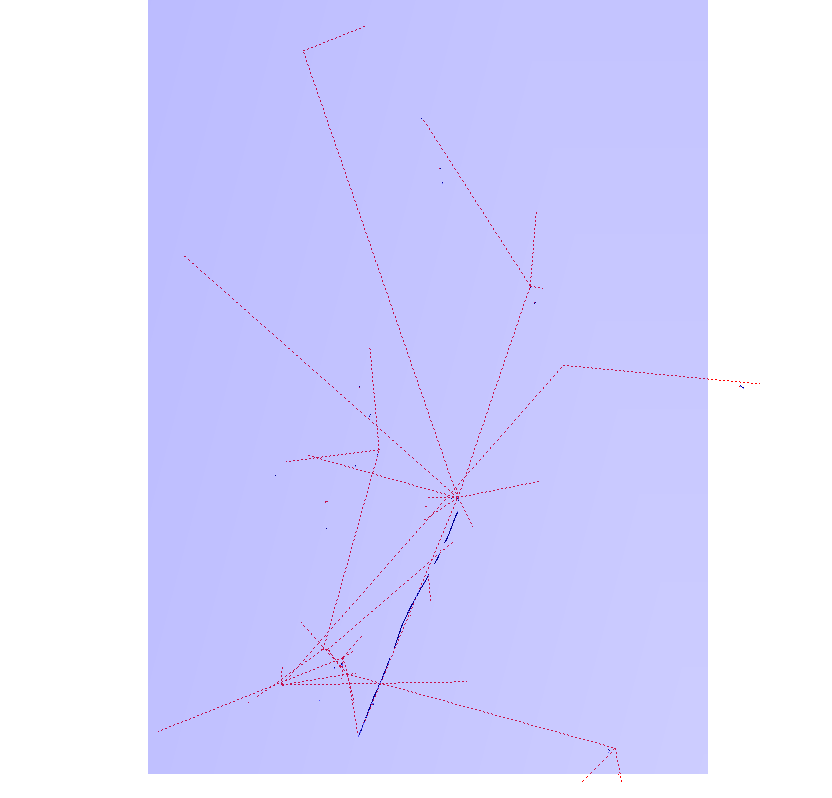
\includegraphics[width=0.5\textwidth]{/var/clus/usera/sv408/pandora_script/calo_and_mc}}
\centering
\caption{Pandora interface with CaloHits (blue) and MCParticles (red)}
\label{fig:calo_and_mc}
\end{figure}

From Figure \ref{fig:calo_and_mc} we can see the CaloHits and the MCParticles. For more examples, see 
\begin{verbatim}
$MY_TEST_AREA/WorkshopContent/examplecontent/ExampleAlgorithms/DisplayListsAlgorithm.cc or .h
\end{verbatim}

\section{Cluster Creationg} \label{sssec:cluster_creation}

A cluster is defined as

Modify MyTestAlgorithm.cc in this way:
\begin{lstlisting}[language=C++, label=code:first_cluster, caption=MyTestAlgorithm.cc creates a basic set of clusters]
#include "Pandora/AlgorithmHeaders.h"
#include "larpandoracontent/LArHelpers/LArClusterHelper.h"
#include "larpandoracontent/LArHelpers/LArMCParticleHelper.h"
#include "workshopcontent/Algorithms/MyTestAlgorithm.h"

using namespace pandora;
using namespace lar_content;

namespace workshop_content
{

MyTestAlgorithm::MyTestAlgorithm():
	m_outputClusterListName(),
	m_nHitsPerCluster(10)
	{
	}

StatusCode MyTestAlgorithm::Run()
{
	//CaloHits
	const CaloHitList *pCaloHitList(nullptr);
	PANDORA_RETURN_RESULT_IF(STATUS_CODE_SUCCESS, !=, PandoraContentApi::GetCurrentList(*this, pCaloHitList));
	
	const ClusterList *pTemporaryList(nullptr);
	std::string temporaryListName;
	PANDORA_RETURN_RESULT_IF(STATUS_CODE_SUCCESS, !=, PandoraContentApi::CreateTemporaryListAndSetCurrent(*this, pTemporaryList, temporaryListName));
	
	CaloHitVector sortedCaloHits(pCaloHitList->begin(), pCaloHitList->end());
	std::sort(sortedCaloHits.begin(), sortedCaloHits.end(), LArClusterHelper::SortHitsByPosition);

	const Cluster *pCluster(nullptr);
	
	for (const CaloHit *const pCaloHit : sortedCaloHits)
	{
		if (!PandoraContentApi::IsAvailable(*this, pCaloHit))
		    continue;
		if (!pCluster || (pCluster->GetNCaloHits() >= m_nHitsPerCluster))
		{
		   PandoraContentApi::Cluster::Parameters parameters;
                   parameters.m_caloHitList.push_back(pCaloHit);
		   PANDORA_RETURN_RESULT_IF(STATUS_CODE_SUCCESS, !=, PandoraContentApi::Cluster::Create(*this, parameters, pCluster));
		}
  		else
 		{
		  PANDORA_RETURN_RESULT_IF(STATUS_CODE_SUCCESS, !=, PandoraContentApi::AddToCluster(*this, pCluster, pCaloHit));
		}
	}
	if (!pTemporaryList->empty())
	{
	   PANDORA_RETURN_RESULT_IF(STATUS_CODE_SUCCESS, !=, PandoraContentApi::SaveList<Cluster>(*this, m_outputClusterListName));
	   PANDORA_RETURN_RESULT_IF(STATUS_CODE_SUCCESS, !=, PandoraContentApi::ReplaceCurrentList<Cluster>(*this, m_outputClusterListName));
	}
	return STATUS_CODE_SUCCESS;
}

StatusCode MyTestAlgorithm::ReadSettings(const TiXmlHandle xmlHandle)
	{
	  PANDORA_RETURN_RESULT_IF(STATUS_CODE_SUCCESS, !=, XmlHelper::ReadValue(xmlHandle, "OutputClusterListName", m_outputClusterListName));
	  PANDORA_RETURN_RESULT_IF_AND_IF(STATUS_CODE_SUCCESS, STATUS_CODE_NOT_FOUND, !=, XmlHelper::ReadValue(xmlHandle,"NHitsPerCluster", m_nHitsPerCluster));
	  return STATUS_CODE_SUCCESS;
	}

}
\end{lstlisting}

change also the MyTestAlgorithm.h

\begin{lstlisting}[language=C++, label=code:first_cluster.h, caption=MyTestAlgorithm.h]
#ifndef WORKSHOP_MYTEST_ALGORITHM_H
#define WORKSHOP_MYTEST_ALGORITHM_H 1

#include "Pandora/Algorithm.h"

namespace workshop_content
{

/**
 *  @brief  MyTestAlgorithm class
 */
class MyTestAlgorithm : public pandora::Algorithm
{
public:
    MyTestAlgorithm();
	
    /**
     *  @brief  Factory class for instantiating algorithm
     */
  
 class Factory : public pandora::AlgorithmFactory
    {
    public:
        pandora::Algorithm *CreateAlgorithm() const;
    };


	
private:
    pandora::StatusCode Run();
    pandora::StatusCode ReadSettings(const pandora::TiXmlHandle xmlHandle);

    // Member variables here

    std::string m_outputClusterListName;
unsigned int m_nHitsPerCluster;

};


inline pandora::Algorithm *MyTestAlgorithm::Factory::CreateAlgorithm() const
{
    return new MyTestAlgorithm();
}

} // namespace workshop_content

#endif // #ifndef WORKSHOP_MYTEST_ALGORITHM_H
\end{lstlisting}

and the PandoraSettings_Workshop.xml

\begin{lstlisting}[language=C++, label=code:first_cluster.xml, caption=PandoraSettings_Workshop.xml]
<pandora>
    <!-- GLOBAL SETTINGS -->
    <IsMonitoringEnabled>true</IsMonitoringEnabled>
    <ShouldDisplayAlgorithmInfo>true</ShouldDisplayAlgorithmInfo>
    <SingleHitTypeClusteringMode>true</SingleHitTypeClusteringMode>

    <!-- ALGORITHM SETTINGS -->
    <algorithm type = "LArEventReading">
        <EventFileNameList>/r05/uboone/jjd49/cincinatti_sample/Pandora_Events_Cincinatti_BNB_NuMu_1714.pndr</EventFileNameList>
        <GeometryFileName>/usera/sv408/WorkshopContent/settings/uboone/Geometry_MicroBooNE.xml</GeometryFileName>
        <SkipToEvent>0</SkipToEvent>
    </algorithm>

    <!-- LAR TPC EVENT RECONSTRUCTION -->
    <algorithm type = "LArListPreparation">
        <OnlyAvailableCaloHits>true</OnlyAvailableCaloHits>
        <OutputCaloHitListNameW>CaloHitListW</OutputCaloHitListNameW>
        <OutputCaloHitListNameU>CaloHitListU</OutputCaloHitListNameU>
        <OutputCaloHitListNameV>CaloHitListV</OutputCaloHitListNameV>
        <FilteredCaloHitListName>CaloHitList2D</FilteredCaloHitListName>
        <CurrentCaloHitListReplacement>CaloHitListW</CurrentCaloHitListReplacement>
        <OutputMCParticleListNameU>MCParticleListU</OutputMCParticleListNameU>
        <OutputMCParticleListNameV>MCParticleListV</OutputMCParticleListNameV>
        <OutputMCParticleListNameW>MCParticleListW</OutputMCParticleListNameW>
        <OutputMCParticleListName3D>MCParticleList3D</OutputMCParticleListName3D>
        <CurrentMCParticleListReplacement>MCParticleListW</CurrentMCParticleListReplacement>
        <MipEquivalentCut>0.</MipEquivalentCut>
    </algorithm>
<!-- parte nuova -->
   <algorithm type = "MyTestAlgorithm">
	<OutputClusterListName>MyFirstClusterW</OutputClusterListName>
    </algorithm>
<!-- fine parte nuova -->
    <algorithm type = "LArVisualMonitoring">
        <CaloHitListNames>CaloHitListW CaloHitListU CaloHitListV</CaloHitListNames>
        <MCParticleListNames>MCParticleList3D</MCParticleListNames>
        <SuppressMCParticles>22:0.01 2112:1.0</SuppressMCParticles>
        <ShowDetector>true</ShowDetector>
	<ClusterListNames>MyFirstClustersW</ClusterListNames>
    </algorithm>
</pandora>
\end{lstlisting}

Now we can understand how the code Listing \ref{code:first_cluster} works. The foundamental idea is that it takes the CaloHits, it sorts it in crescent order of z-coordinate, it than creates a cluster, it fills the cluster with the first 10 CaloHits, it then create a new cluster and re-iterate the process. 
\begin{lstlisting}[language=C++]
MyTestAlgorithm::MyTestAlgorithm():
	m_outputClusterListName(),
	m_nHitsPerCluster(10)
\end{lstlisting}
It defines and initialises variabiles, in particular says that m${\_}$nHitsPerCluster, the maximun number of CaloHits per cluster, is 10. 

\begin{lstlisting}[language=C++]
	const CaloHitList *pCaloHitList(nullptr);
	PANDORA_RETURN_RESULT_IF(STATUS_CODE_SUCCESS, !=, PandoraContentApi::GetCurrentList(*this, pCaloHitList));
\end{lstlisting}
In the first line you typedef CaloHitList std::list::<CaloHit>. So you define a new list of CaloHit named pCaloHitList and you initialise to zero. The second line says: "using PandoraContentApi, get from the file a list of CaloHits. If this operation is not success (the status code is different from the success status code) exit the program."

\begin{lstlisting}[language=C++]	
	const ClusterList *pTemporaryList(nullptr);
	std::string temporaryListName;
	PANDORA_RETURN_RESULT_IF(STATUS_CODE_SUCCESS, !=, PandoraContentApi::CreateTemporaryListAndSetCurrent(*this, pTemporaryList, temporaryListName));
\end{lstlisting}

First line same thing as before, creating a list of clusters named pTemporaryList. Third line you say: "using PandoraContentApi, create a new list and set it current. If it does not work, exit the programm".

\begin{lstlisting}[language=C++]
	CaloHitVector sortedCaloHits(pCaloHitList->begin(), pCaloHitList->end());
	std::sort(sortedCaloHits.begin(), sortedCaloHits.end(), LArClusterHelper::SortHitsByPosition);
\end{lstlisting}

It sorts CaloHits according to z coordinate.

\begin{lstlisting}[language=C++]
const Cluster *pCluster(nullptr);
\end{lstlisting}

It defines and initialises pCluster.

\begin{lstlisting}[language=C++]
	for (const CaloHit *const pCaloHit : sortedCaloHits)
	{
		if (!PandoraContentApi::IsAvailable(*this, pCaloHit))
		    continue;
\end{lstlisting}
For every CaloHit you have after been sorted. If you see that that CaloHit has already been counted, continue. In this case, continue means skip that CaloHit and go to the other one.
\begin{lstlisting}[language=C++]
		if (!pCluster || (pCluster->GetNCaloHits() >= m_nHitsPerCluster))
		{
		   PandoraContentApi::Cluster::Parameters parameters;
                   parameters.m_caloHitList.push_back(pCaloHit);
		   PANDORA_RETURN_RESULT_IF(STATUS_CODE_SUCCESS, !=, PandoraContentApi::Cluster::Create(*this, parameters, pCluster));
		}
  		else
 		{
		  PANDORA_RETURN_RESULT_IF(STATUS_CODE_SUCCESS, !=, PandoraContentApi::AddToCluster(*this, pCluster, pCaloHit));
		}
	}
\end{lstlisting}
If you do not have a cluster or the cluster is already filled with more CaloHits than the defined maximum number (in this case 10), create a new cluster and put CaloHit into it. Otherwise add to the cluster.
\begin{lstlisting}[language=C++]
	if (!pTemporaryList->empty())
	{
	   PANDORA_RETURN_RESULT_IF(STATUS_CODE_SUCCESS, !=, PandoraContentApi::SaveList<Cluster>(*this, m_outputClusterListName));
	   PANDORA_RETURN_RESULT_IF(STATUS_CODE_SUCCESS, !=, PandoraContentApi::ReplaceCurrentList<Cluster>(*this, m_outputClusterListName));
	}
	return STATUS_CODE_SUCCESS;
}
\end{lstlisting}
Quando hai finito la list, salvala.

\begin{lstlisting}[language=C++]
\end{lstlisting}

\begin{lstlisting}[language=C++]
\end{lstlisting}


\afterpage{\null\newpage}
	\chapter{Cluster Merging}

In this section we will see different examples of meging codes for clusters.

\section{First Cluster Merging Algorithm} \label{sssec:first_merging}
\subsection{CC and Header file} \label{sssec:first_merging_ccandh}
We have to write a new algorithm called MyClusterMergingAlgorithm, and therefore as first thing we havew to run:
\begin{verbatim}
python CreateNewAlgorithm.py --name MyClusterMerging
\end{verbatim}
At this point modify MyMergingAlgorithm.cc as it follows:
\begin{lstlisting}[language=C++,caption=MyClusterMergingAlgorithm.cc]
#include "Pandora/AlgorithmHeaders.h"
#include "larpandoracontent/LArHelpers/LArClusterHelper.h"
#include "larpandoracontent/LArHelpers/LArMCParticleHelper.h"
#include "workshopcontent/Algorithms/MyClusterMergingAlgorithm.h"

using namespace pandora;
using namespace lar_content;

namespace workshop_content
{
MyClusterMergingAlgorithm::MyClusterMergingAlgorithm():
	m_inputClusterListName(),
	m_minClusterCaloHits(1),// THESE ARE RANDOM NUMBERS USED TO SHOW HOW IT WORKS
	m_maxClusterSeparation(10)//
{
}

void MyClusterMergingAlgorithm::GetSortedLongClusters(const ClusterList *const pClusterList, ClusterVector &sortedLongClusters) const
{
	for (const Cluster *const pCluster : *pClusterList)
	{
		if (pCluster->GetNCaloHits() > m_minClusterCaloHits)
		sortedLongClusters.push_back(pCluster);
	}
	std::sort(sortedLongClusters.begin(), sortedLongClusters.end(), LArClusterHelper::SortByNHits);
}

bool MyClusterMergingAlgorithm::AreClustersAssociated(const Cluster *const pParentCluster, const Cluster *const pDaughterCluster) const
{
	// TODO This is where the crucial cluster-merging decision is to be made - add sophistication here!
	if (LArClusterHelper::GetClosestDistance(pParentCluster, pDaughterCluster) > m_maxClusterSeparation)
	 return false;

	return true;
}


StatusCode MyClusterMergingAlgorithm::Run()
{
	const ClusterList *pClusterList(nullptr);
	PANDORA_RETURN_RESULT_IF(STATUS_CODE_SUCCESS, !=, PandoraContentApi::GetList(*this, m_inputClusterListName, pClusterList));

	ClusterVector sortedLongClusters;
	this->GetSortedLongClusters(pClusterList, sortedLongClusters);

	ClusterList defunctClusters;
	
	for (const Cluster *const pParentCluster : sortedLongClusters)
	{
 
bool isInListParent(std::find(defunctClusters.begin(), defunctClusters.end(), pParentCluster) != defunctClusters.end());

if (isInListParent) continue;
		
		for (const Cluster *const pDaughterCluster : sortedLongClusters)
		{
bool isInListDaughter(std::find(defunctClusters.begin(), defunctClusters.end(), pDaughterCluster) != defunctClusters.end());
			if ((pParentCluster == pDaughterCluster) || (isInListDaughter))
			continue;
			
			if (!this->AreClustersAssociated(pParentCluster, pDaughterCluster))
			continue;

			PANDORA_RETURN_RESULT_IF(STATUS_CODE_SUCCESS, !=, PandoraContentApi::MergeAndDeleteClusters(*this, pParentCluster, pDaughterCluster));
			defunctClusters.push_back(pDaughterCluster);
		}

	}
	return STATUS_CODE_SUCCESS;
}
StatusCode MyClusterMergingAlgorithm::ReadSettings(const TiXmlHandle xmlHandle)
	{
	  PANDORA_RETURN_RESULT_IF(STATUS_CODE_SUCCESS, !=, XmlHelper::ReadValue(xmlHandle, "InputClusterListName", m_inputClusterListName));
	  return STATUS_CODE_SUCCESS;
	}
}
\end{lstlisting}
This code takes all the clusters, it sorts them, it define a cluster parent and a daughter and it checks the distance between those 2. If the distance is higher than a certain number it will not merge them together otherwise it will. Now let's go through all the important parts of this file.

\begin{lstlisting}[language=C++]
void MyClusterMergingAlgorithm::GetSortedLongClusters(const ClusterList *const pClusterList, ClusterVector &sortedLongClusters) const
{
	for (const Cluster *const pCluster : *pClusterList)
	{
		if (pCluster->GetNCaloHits() > m_minClusterCaloHits)
		sortedLongClusters.push_back(pCluster);
	}
	std::sort(sortedLongClusters.begin(), sortedLongClusters.end(), LArClusterHelper::SortByNHits);
}
\end{lstlisting}
GetSortedLongClusters is a function of MyClusterMergingAlgorithm that if the number of CaloHits contained\\ is bigger than a certain number m${\_}$minClusterCaloHits, it puts that cluster at the end of the list sortedLongClusters. Than, starting from the first element of that list until the last one, those clusters are sorted according to the number of CaloHits in each cluster.
\begin{lstlisting}[language=C++]
bool MyClusterMergingAlgorithm::AreClustersAssociated(const Cluster *const pParentCluster, const Cluster *const pDaughterCluster) const
{
	// TODO This is where the crucial cluster-merging decision is to be made - add sophistication here!
	if (LArClusterHelper::GetClosestDistance(pParentCluster, pDaughterCluster) > m_maxClusterSeparation)
	 return false;

	return true;
}
\end{lstlisting}
AreClusterAssociated is the foundamental function to decide wheter a cluster should be merged or not. In this case, if the distance between two clusters is smaller than m${\_}$maxClusterSeparation, AreClusterAssociated will be true.
\begin{lstlisting}[language=C++]
	const ClusterList *pClusterList(nullptr);
	PANDORA_RETURN_RESULT_IF(STATUS_CODE_SUCCESS, !=, PandoraContentApi::GetList(*this, m_inputClusterListName, pClusterList));

	ClusterVector sortedLongClusters;
	this->GetSortedLongClusters(pClusterList, sortedLongClusters);

\end{lstlisting}

In this part the cluster list is read from the input file and saved in the pClusterList, at the beginning initialised to a null pointer. Those clusters are then sorted.

\begin{lstlisting}[language=C++]
ClusterList defunctClusters;
	
	for (const Cluster *const pParentCluster : sortedLongClusters)
	{
 
bool isInListParent(std::find(defunctClusters.begin(), defunctClusters.end(), pParentCluster) != defunctClusters.end());

if (isInListParent) continue;
\end{lstlisting}

A list defunctClusters is defined, that is the list of Clusters which have already been used (at this stage the list is empty). Then it starts a for-cicle over all the the sorted Clusters in sortedLongClusters. The standard definition is the following:

\begin{verbatim}
for(type name: where)
\end{verbatim} 
in this case the type is const Cluster *const, the name of the current element is pParentCluster and where is sortedLongCLuster. Then we have the bool function isInListParent. It works like that: if pParentCluster is in defunctClusters list it returns true. It searches pParentCluster from begin to end, where end is one step forward the last occupied cluster. If the pParentCluster is not found, by default it said that it lives in defunctCluster.end. If isInListParent is true, than that pParentCluster is skipped, because it means it has already been used.
\begin{lstlisting}[language=C++]
for (const Cluster *const pDaughterCluster : sortedLongClusters)
		{
bool isInListDaughter(std::find(defunctClusters.begin(), defunctClusters.end(), pDaughterCluster) != defunctClusters.end());
			if ((pParentCluster == pDaughterCluster) || (isInListDaughter))
			continue;
\end{lstlisting}
You do the same things for the pDaughterCluster plus you request to take clusters which where not pParentCluster. Basically you take a pParentCluster and then you get a list of other pDaughter which have not previously used.

\begin{lstlisting}[language=C++]
			if (!this->AreClustersAssociated(pParentCluster, pDaughterCluster))
			continue;

			PANDORA_RETURN_RESULT_IF(STATUS_CODE_SUCCESS, !=, PandoraContentApi::MergeAndDeleteClusters(*this, pParentCluster, pDaughterCluster));
			defunctClusters.push_back(pDaughterCluster);
		}

	}
	return STATUS_CODE_SUCCESS;
\end{lstlisting}

If AreClustersAssociated is not true (the distance is bigger than the max distance), skip that daughter, otherwise merge the cluster and put pDaughterCluster in defunctClusters.\\
We have then to modify accordingly the header file.

\begin{lstlisting}[language=C++, caption=MyClusterMergingAlgorithm.h]
#ifndef WORKSHOP_MYCLUSTERMERGING_ALGORITHM_H
#define WORKSHOP_MYCLUSTERMERGING_ALGORITHM_H 1

#include "Pandora/Algorithm.h"

namespace workshop_content
{

/**
 *  @brief  MyClusterMergingAlgorithm class
 */
class MyClusterMergingAlgorithm : public pandora::Algorithm
{
public:
    MyClusterMergingAlgorithm();
	
    /**
     *  @brief  Factory class for instantiating algorithm
     */
  
 class Factory : public pandora::AlgorithmFactory
    {
    public:
        pandora::Algorithm *CreateAlgorithm() const;
    };


	
private:
    pandora::StatusCode Run();
    pandora::StatusCode ReadSettings(const pandora::TiXmlHandle xmlHandle);

    // Member variables here
 void GetSortedLongClusters(const pandora::ClusterList *const pClusterList, pandora::ClusterVector &sortedLongClusters) const;
 bool AreClustersAssociated(const pandora::Cluster *const pParentCluster, const pandora::Cluster *const pDaughterCluster) const;


 std::string m_inputClusterListName;
 unsigned int m_minClusterCaloHits;
 unsigned int m_maxClusterSeparation;

};


inline pandora::Algorithm *MyClusterMergingAlgorithm::Factory::CreateAlgorithm() const
{
    return new MyClusterMergingAlgorithm();
}

} // namespace workshop_content

#endif // #ifndef WORKSHOP_MYCLUSTERMERGING_ALGORITHM_H
\end{lstlisting}
Then, we have to modify PandoraSettings${\_}$Workshop.xml from the version from
\begin{lstlisting}[language=XML, caption=Previous version of PandoraSettings${\_}$Workshop.xml]
<pandora>
    <!-- GLOBAL SETTINGS -->
    <IsMonitoringEnabled>true</IsMonitoringEnabled>
    <ShouldDisplayAlgorithmInfo>true</ShouldDisplayAlgorithmInfo>
    <SingleHitTypeClusteringMode>true</SingleHitTypeClusteringMode>

    <!-- ALGORITHM SETTINGS -->
    <algorithm type = "LArEventReading">
        <EventFileNameList>/r05/uboone/jjd49/cincinatti_sample/Pandora_Events_Cincinatti_BNB_NuMu_1714.pndr</EventFileNameList>
        <GeometryFileName>/usera/sv408/WorkshopContent/settings/uboone/Geometry_MicroBooNE.xml</GeometryFileName>
        <SkipToEvent>0</SkipToEvent>
    </algorithm>
    <!-- LAR TPC EVENT RECONSTRUCTION -->
    <algorithm type = "LArListPreparation">
        <OnlyAvailableCaloHits>true</OnlyAvailableCaloHits>
        <OutputCaloHitListNameW>CaloHitListW</OutputCaloHitListNameW>
        <OutputCaloHitListNameU>CaloHitListU</OutputCaloHitListNameU>
        <OutputCaloHitListNameV>CaloHitListV</OutputCaloHitListNameV>
        <FilteredCaloHitListName>CaloHitList2D</FilteredCaloHitListName>
        <CurrentCaloHitListReplacement>CaloHitListW</CurrentCaloHitListReplacement>
        <OutputMCParticleListNameU>MCParticleListU</OutputMCParticleListNameU>
        <OutputMCParticleListNameV>MCParticleListV</OutputMCParticleListNameV>
        <OutputMCParticleListNameW>MCParticleListW</OutputMCParticleListNameW>
        <OutputMCParticleListName3D>MCParticleList3D</OutputMCParticleListName3D>
        <CurrentMCParticleListReplacement>MCParticleListW</CurrentMCParticleListReplacement>
        <MipEquivalentCut>0.</MipEquivalentCut>
    </algorithm>

   <algorithm type = "MyTestAlgorithm">
	<OutputClusterListName>MyFirstClusterW</OutputClusterListName>
    </algorithm>

    <algorithm type = "LArVisualMonitoring">
        <CaloHitListNames>CaloHitListW CaloHitListU CaloHitListV</CaloHitListNames>
        <MCParticleListNames>MCParticleList3D</MCParticleListNames>
        <SuppressMCParticles>22:0.01 2112:1.0</SuppressMCParticles>
        <ShowDetector>true</ShowDetector>
	<ClusterListNames>MyFirstClustersW</ClusterListNames>
    </algorithm>
</pandora>
\end{lstlisting}

to 

\begin{lstlisting}[language=XML, caption=New version of PandoraSettings${\_}$Workshop.xml]
<pandora>
    <!-- GLOBAL SETTINGS -->
    <IsMonitoringEnabled>true</IsMonitoringEnabled>
    <ShouldDisplayAlgorithmInfo>true</ShouldDisplayAlgorithmInfo>
    <SingleHitTypeClusteringMode>true</SingleHitTypeClusteringMode>

    <!-- ALGORITHM SETTINGS -->
    <algorithm type = "LArEventReading">
        <EventFileNameList>/r05/uboone/jjd49/cincinatti_sample/Pandora_Events_Cincinatti_BNB_NuMu_1714.pndr</EventFileNameList>
        <GeometryFileName>/usera/sv408/WorkshopContent/settings/uboone/Geometry_MicroBooNE.xml</GeometryFileName>
        <SkipToEvent>0</SkipToEvent>
    </algorithm>

    <!-- LAR TPC EVENT RECONSTRUCTION -->
    <algorithm type = "LArListPreparation">
        <OnlyAvailableCaloHits>true</OnlyAvailableCaloHits>
        <OutputCaloHitListNameW>CaloHitListW</OutputCaloHitListNameW>
        <OutputCaloHitListNameU>CaloHitListU</OutputCaloHitListNameU>
        <OutputCaloHitListNameV>CaloHitListV</OutputCaloHitListNameV>
        <FilteredCaloHitListName>CaloHitList2D</FilteredCaloHitListName>
        <CurrentCaloHitListReplacement>CaloHitListW</CurrentCaloHitListReplacement>
        <OutputMCParticleListNameU>MCParticleListU</OutputMCParticleListNameU>
        <OutputMCParticleListNameV>MCParticleListV</OutputMCParticleListNameV>
        <OutputMCParticleListNameW>MCParticleListW</OutputMCParticleListNameW>
        <OutputMCParticleListName3D>MCParticleList3D</OutputMCParticleListName3D>
        <CurrentMCParticleListReplacement>MCParticleListW</CurrentMCParticleListReplacement>
        <MipEquivalentCut>0.</MipEquivalentCut>
    </algorithm>

<algorithm type = "LArClusteringParent">
<algorithm type = "LArTrackClusterCreation" description = "ClusterFormation"/>
<InputCaloHitListName>CaloHitListW</InputCaloHitListName>
<ClusterListName>MyFirstClustersW</ClusterListName>
<ReplaceCurrentCaloHitList>false</ReplaceCurrentCaloHitList>
<ReplaceCurrentClusterList>true</ReplaceCurrentClusterList>
</algorithm>

 <algorithm type = "LArVisualMonitoring">
<CaloHitListNames>CaloHitListW</CaloHitListNames>
<ClusterListNames>MyFirstClustersW</ClusterListNames>
</algorithm>
</pandora>

<algorithm type = "MyClusterMerging">
<InputClusterListName>MyFirstClustersW</InputClusterListName>
</algorithm>

<algorithm type = "LArVisualMonitoring"> 
<ClusterListNames>MyFirstClustersW</ClusterListNames> 
</algorithm> 

</pandora>

\end{lstlisting}

The idea is that we want to visualise the clusters when they are not merged together and when they are. With

\begin{lstlisting}[language=XML]
<algorithm type = "LArClusteringParent">
<algorithm type = "LArTrackClusterCreation" description = "ClusterFormation"/>
<InputCaloHitListName>CaloHitListW</InputCaloHitListName>
<ClusterListName>MyFirstClustersW</ClusterListName>
<ReplaceCurrentCaloHitList>false</ReplaceCurrentCaloHitList>
<ReplaceCurrentClusterList>true</ReplaceCurrentClusterList>
</algorithm>
\end{lstlisting}

LArClusteringParent is an algorithm which controls that any CaloHit has not taken or counted twice. LArTrackClusterCreation is the actual logic that fills the clusters with the CaloHits. Then it follows LArVisualMonitoring to visualise the clusters. Then we have:  

\begin{lstlisting}[language=XML]
<algorithm type = "MyClusterMerging">
<InputClusterListName>MyFirstClustersW</InputClusterListName>
</algorithm>

<algorithm type = "LArVisualMonitoring"> 
<ClusterListNames>MyFirstClustersW</ClusterListNames> 
</algorithm> 
\end{lstlisting}
which calls my new algorithm MyClusterMerging and visualises it. Now it will be shown a first example of mergin algorithm.
\begin{figure}[h]
\scalebox{0.25}{\includegraphics[width=0.5\textwidth]{/var/clus/usera/sv408/pandora_script/cluster1_cropped}}
\centering
\caption{Set of clusters before merging algorithm}
\label{fig:cluster1}
\end{figure}

\begin{figure}[h]
\scalebox{0.25}{\includegraphics[width=0.5\textwidth]{/var/clus/usera/sv408/pandora_script/cluster2_cropped}}
\centering
\caption{Set of merged clusters after merging algorithm}
\label{fig:cluster2}
\end{figure}

\section{Merging Algorithm Using LArPointerCluster} \label{sssec:larpointer_cluster}
To use a more sofisticated tool, substitute in AreClustersAssociated: 

\begin{lstlisting}[language=C++]
bool MyClusterMergingAlgorithm::AreClustersAssociated(const Cluster *const pParentCluster, const Cluster *const pDaughterCluster) const
{
	try
	{
	// Useful constructs for pointing information
		const LArPointingCluster parentPointingCluster(pParentCluster);
		const LArPointingCluster daughterPointingCluster(pDaughterCluster);
		LArPointingCluster::Vertex closestVertexParent, closestVertexDaughter;
		LArPointingClusterHelper::GetClosestVertices(parentPointingCluster, daughterPointingCluster, closestVertexParent, closestVertexDaughter);
		// Impact parameters
		float parentDaughterImpactL(std::numeric_limits<float>::max()), parentDaughterImpactT(std::numeric_limits<float>::max());
		LArPointingClusterHelper::GetImpactParameters(closestVertexParent, closestVertexDaughter, parentDaughterImpactL, parentDaughterImpactT);
		float daughterParentImpactL(std::numeric_limits<float>::max()), daughterParentImpactT(std::numeric_limits<float>::max());
		LArPointingClusterHelper::GetImpactParameters(closestVertexDaughter, closestVertexParent, daughterParentImpactL, daughterParentImpactT);
		// Visualization and debug
		std::cout << "MyClusterMergingAlgorithm::AreClustersAssociated " << std::endl;
		std::cout << "parentDaughterImpactL: " << parentDaughterImpactL << ", parentDaughterImpactT " << parentDaughterImpactT << std::endl;
		std::cout << "daughterParentImpactL: " << daughterParentImpactL << ", daughterParentImpactT " << daughterParentImpactT << std::endl;
		ClusterList parentList, daughterList;
		parentList.push_back(pParentCluster); daughterList.push_back(pDaughterCluster);
		PandoraMonitoringApi::VisualizeClusters(this->GetPandora(), &parentList, "ParentCluster", RED);
		PandoraMonitoringApi::VisualizeClusters(this->GetPandora(), &daughterList, "DaughterCluster", BLUE);
		PandoraMonitoringApi::AddMarkerToVisualization(this->GetPandora(), &(closestVertexParent.GetPosition()), "ParentVertex", ORANGE, 2);
		PandoraMonitoringApi::AddMarkerToVisualization(this->GetPandora(), &(closestVertexDaughter.GetPosition()), "DaughterVertex", GREEN, 2);
		PandoraMonitoringApi::ViewEvent(this->GetPandora());
		// Make decision
		if (((parentDaughterImpactL < m_maxImpactL) && (parentDaughterImpactT < m_maxImpactT)) || ((daughterParentImpactL < m_maxImpactL) && (daughterParentImpactT < m_maxImpactT)))
		{
			return true;
		}
	}
	catch (const StatusCodeException &statusCodeException)
	{
		std::cout << "MyClusterMergingAlgorithm::AreClustersAssociated " << statusCodeException.ToString() << std::endl;
	}
	return false;
}
\end{lstlisting}

and remeber to add

\begin{lstlisting}
#include "larpandoracontent/LArHelpers/LArPointingClusterHelper.h"
\end{lstlisting}




\afterpage{\null\newpage}
	\input{/home/stefano/Documents/fermilab/thesis/chapter5/chapter5}
\afterpage{\null\newpage}



	\backmatter
%\include{glossary}
%\include{notat}
	\bibliographystyle{amsalpha} %The style you want to use for references.
%\bibliography{mr,refs} %The files containing all the articles and books you ever referenced.
	\printindex %Make an index AUTOMATICALLY

	\addcontentsline{toc}{section}{References}
  	\begin{thebibliography}{1}

		\bibitem{t2} T. Doke et al. {\em Let Dependence of Scintillation Yield In Liquid Argon}. Nuclear Instruments and Methods in Physics Research {\textbf {A269}} pagg. 291-296, 1988. 
		\bibitem{t1} C. Amsler et al. {\em Luminescence quenching of the triplet excimer state by air traces in gaseous argon}. arXiv:0708.2621v1.
		\bibitem{t3} R. Acciarri et al. {\em Effects of Nitrogen contamination in liquid Argon}. arXiv:0804.1217.
		\bibitem{chiu} Christie Shinglei Chiu {\em Liquid Argon Scintillation Light Quenching due to Nitrogen Impurities: Measurements performed for the MicroBooNE Vertical Slice Test} Bachelor Thesis, MIT, id.numb. 865477653, June 2013.
		\bibitem{t4} D. Whittington, S. Mufson and B. Howard {\em Scintillation Light from Cosmic-Ray Muons in Liquid Argon}. arXiv:1408.1763v5.
		\bibitem{janet} R. Jerry, L. Winslow, L. Bugel and J.M. Conrad {\em A Study of the Fluorescence Response of Tetraphenyl-butadiene}. arXiv:1411.4524v2.
		\bibitem{segreto} E. Segreto {\em Evidence of delayed light emission of TetraPhenyl Butadiene excited by liquid Argon scintillation light}. arXiv:1411.4524v2. 
		\bibitem{tpb} http://www.tcichemicals.com/eshop/en/us/commodity/T0168/.
		\bibitem{einstein} A. Einstein {\em \"Uber einen die Erzeugung und Verwandlung des Lichtes betreffenden heuristichen Gesichtspunkt}. Annalen der Physik {\textbf {17}}, pagg. 132-148, 1905.
		\bibitem{wiki1} {\em Wikipedia: Depletion Region}, September 2016.
		\bibitem{silicon} V. Saveliev {\em Silicon Photomultiplier - New Era of Photon Detection} Advances in Optical and Photonic Devices, Ki Young Kim (Ed.), InTech, DOI: 10.5772/7150. Available from: http://www.intechopen.com/books/advances-in-optical-and-photonic-devices/silicon-photomultiplier-new-era-of-photon-detection, 2010.
		\bibitem{impact} S.M. Sze {\em Physics of Semiconductor Devices}. John Wiley \& Sons. p. 45. ISBN 0-471-05661-8. 1981.
		\bibitem{guide1} {\em An Introduction to the Silicon Photomultiplier}. http://www.sensl.com/downloads/ds/TN\%20-\%20Intro\%20to\%20SPM\%20Tech.pdf, September 2016.
  		\bibitem{sensl} http://sensl.com/downloads/ds/DS-MicroCseries.pdf, September 2016.
  		\bibitem{sensl2} http://sensl.com/estore/microfc-60035-smt/, September 2016.
		\bibitem{hamamatsu} http://www.hamamatsu.com/resources/pdf/ssd/s13360${\_}$series${\_}$kapd1052e.pdf, September 2016.
		\bibitem{hamamatsu2} http://www.hamamatsu.com/jp/en/S13360-3050CS.html, September 2016.
		\bibitem{omega} {\em What is a Thermoresistor?} http://www.omega.com/prodinfo/thermistor.html, September 2016.
		\bibitem{power_supply} Lambda Power Supply spec sheet - http://prep.fnal.gov/catalog/hardware${\_}$info/lambda/lpd425afm.html, September 2016.
		\bibitem{preamp} Spec Sheet Pre Amplifier - http://www.mech-tronics.com/f${\_}$ni400.htm, September 2016.
		\bibitem{amp} Spec Sheet Amplifier - http://www.mech-tronics.com/f${\_}$ni511.htm, September 2016.
		\bibitem{wikiexpo} Wikipedia's page : Exponentially Modified Gaussian Distribution - https://en.wikipedia.org/wiki/Exponentially${\_}$modified${\_}$Gaussian${\_}$distribution, September 2016.
  	\end{thebibliography}

	\appendix
%\addcontentsline{toc}{chapter}{Appendix}
	\addtocontents{toc}{\protect\contentsline{chapter}{Appendix:}{}}
	\chapter{Hamamatsu MPPCs}\label{sssec:mppc}
	\includepdf[pages=-]{/home/stefano/Documents/fermilab/thesis/pictures/s13360_series_kapd1052e.pdf}
	\chapter{Diodes}\label{sssec:diode1}
	\includepdf[pages=-]{/home/stefano/Documents/fermilab/thesis/pictures/diode1.pdf}
	\includepdf[pages=-]{/home/stefano/Documents/fermilab/thesis/pictures/diode2.pdf}
	

  	\end{document}
